\section{Experiment 2 : influence of the parameter s.}
For the second experiment, we use the following parameter settings : 
\begin{table}[h]
\centering
\begin{tabular}{lll}
    $ R_0 = 1000, $  &  $ f_{gen} = 0.1, $ & $ f_{noise} = 0.6 ,$  \\
    $ \sigma_{i_0} = 0.1, $  &  $ \sigma_{n_i} = 0.1, $ & $ \sigma_{n_u} = 1.$  \\
\end{tabular}
\end{table}

The purpose here is to analyze the influence of the shift $s$ on the estimation by making it vary ($s = 1, 2$ and $5$) with constant filters. The results are displayed on figure \ref{fig: Sess1_part1_exp2}. Moreover, the most important results are visible in table \ref{tab: Sess1_part1_exp2}. 

As we increase the shift $s$, we can see that $\hat{R}_{IV}$ becomes closer to the searched value $R_0 = 1000$, i.e. the bias becomes smaller. This is because the ratio $R_{n_i n_i}(s)/R_{i_0 i_0}(s)$ becomes smaller with increasing $s$ (cfr. table \ref{tab: Sess1_part1_exp2}). We observe that the sign of the bias depends on the sign of $R_{n_i n_i}(s)$. This can be seen by looking at equation~\ref{as_val_IV} : if $R_{n_i n_i}(s) \ge 0$, the factor $(1+R_{n_i n_i}(s)/R_{i_0 i_0}(s))^{-1}$ is smaller than 1, which results in an under-estimation of $R_0$. At the other hand, if $R_{n_i n_i}(s) \le 0$, a similar reasoning leads to the conclusion that $R_0$ will be over-estimated. That is indeed what we observe in table~\ref{tab: Sess1_part1_exp2}.

\begin{table}[ht]
\centering
\begin{tabular}{|c|c|c|c|c|c|}
\hline
$s$ & $R_{n_i n_i}(s)$ & $R_{i_0 i_0}(s)$ & $R_{n_i n_i}(s)/R_{i_0 i_0}(s)$ & theoretical $\hat{R}_{IV}$ & experimental $\hat{R}_{IV}$ \\
\hline
\hline
1 & 0.0048 & 0.0086 & 0.5532 & 634 & $\mu$ = 645.44\\
\hline
2 & -0.0012 & 0.0062 & -0.1953 & 1242 & $\mu$ = 1226.5 \\
\hline
5 & -0.0001 & 0.0021 & -0.0435 & 1045 & $\mu$ = 1039.33 \\
\hline
\end{tabular}\caption{}\label{tab: Sess1_part1_exp2}
\end{table}
However, the IV estimates does not seem to be the perfect choice since its variance keeps increasing with $s$. This is mainly due to the auto-correlation function of the current $R_{i_0 i_0}(s)$  that becomes smaller with increasing shift $s$. We can compute an approximation of the variance by neglecting the second order terms and by doing a Taylor series expansion. This leads to :
\begin{equation}
\lim\limits_{N \rightarrow +\infty} \sigma^2_{\hat{R}_{IV}} = \sigma^2_{n_u} \frac{\sigma^2_{n_i}  + \sigma^2_{i_0}}{(R_{n_i n_i}(s) + R_{i_0 i_0}(s))^2}
\end{equation}


\begin{figure}[H]
    \centering
    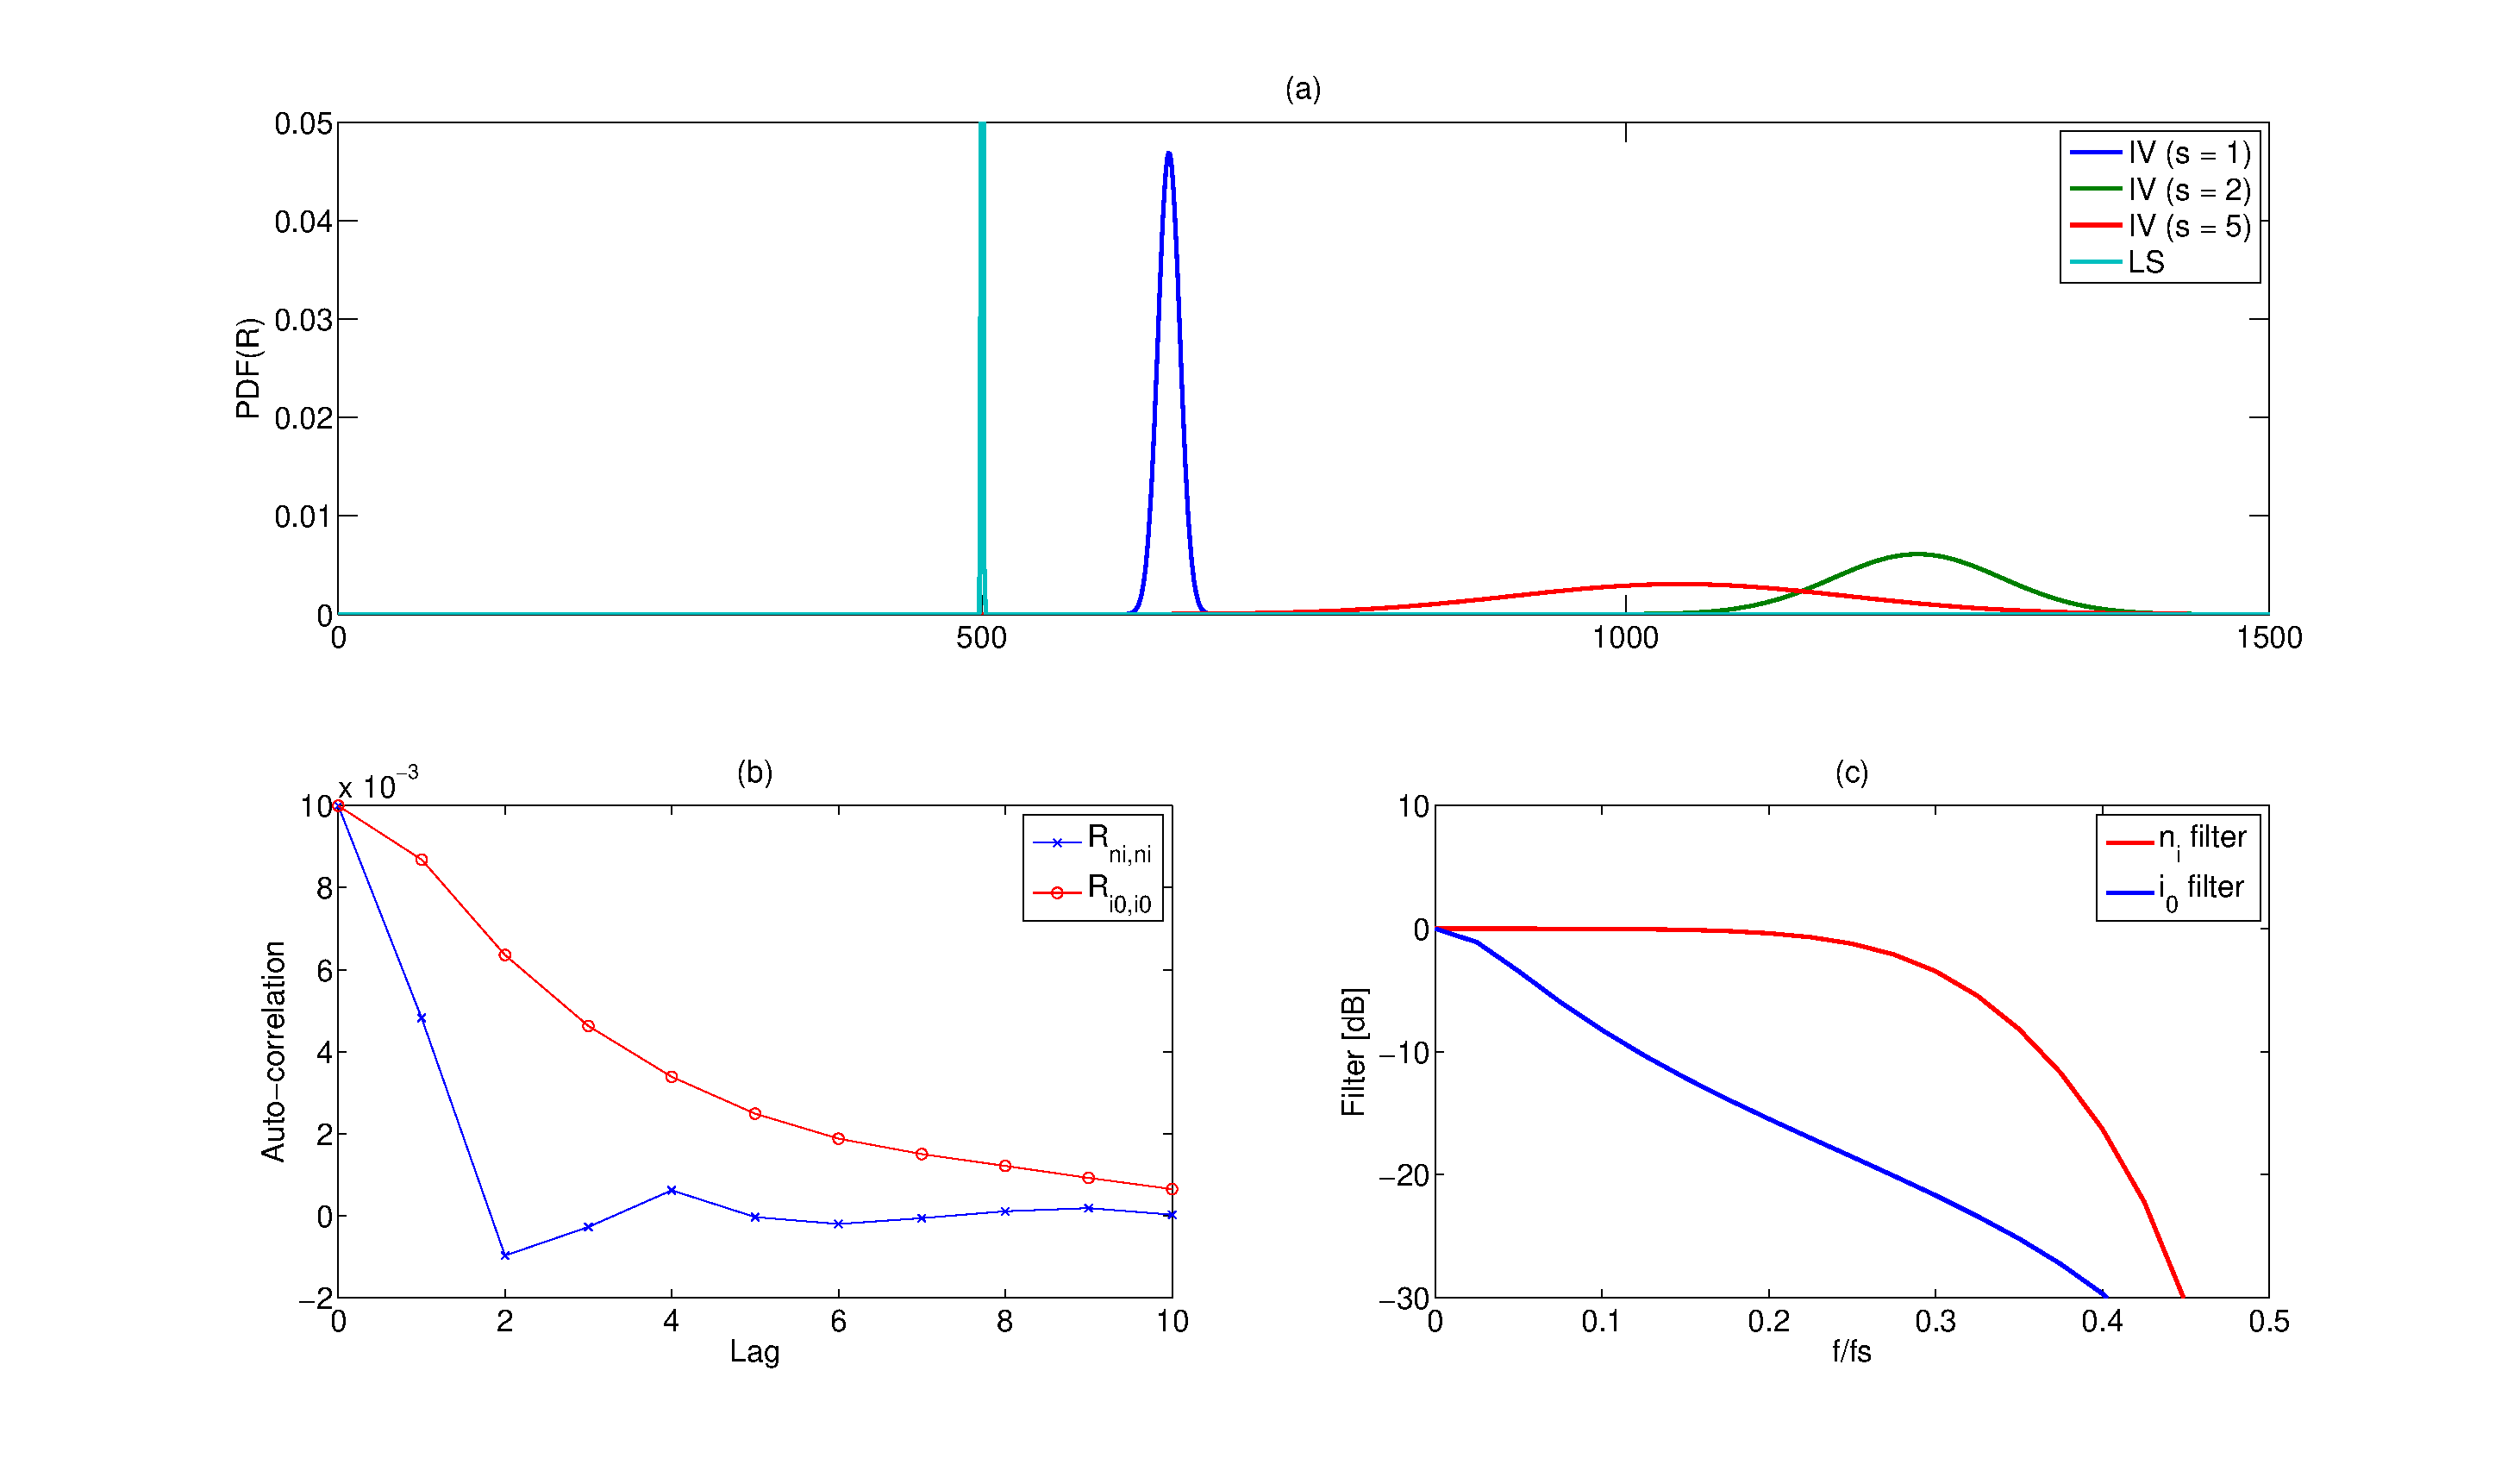
\includegraphics[width=1\textwidth]{Figures/Sess1_part1_exp2.eps}
    \caption{Study of the LS and IV estimates for a fixed noise filter bandwidth and varying shift parameter $s =$ {1, 2, 5}. Fig. (a) : the LS (cyan) and IV estimates. IV(1) (blue), IV(2) (green) and IV(3) (red) correspond to a shift of 1, 2 and 5 respectively. Fig. (b): the auto-correlation of $i_0$ (red) and $n_i$ (blue). Fig. (c) : filter characteristics of $i_0$ (blue) and of $n_i$ (red).}
    \label{fig: Sess1_part1_exp2}
\end{figure}
